%%%%%%%%%%%%%%%%%%%%%%%%%%%%%%%%%%%%%%%%%%%%%%%%%%%%%%%%%%%%
%%%%%%%%%%%%%%%%%%%%%%%%%%%%%%%%%%%%%%%%%%%%%%%%%%%%%%%%%%%%
\chapter{Defining the Potential}
\label{chap:pot}
\nopagebreak
%%%%%%%%%%%%%%%%%%%%%%%%%%%%%%%%%%%%%%%%%%%%%%%%%%%%%%%%%%%%
%%%%%%%%%%%%%%%%%%%%%%%%%%%%%%%%%%%%%%%%%%%%%%%%%%%%%%%%%%%%



In Chapter~\ref{chap:alg}, we have seen that it is possible to map all the
possible sequences with the correct total mass on the configurations of a
physical model with discrete variables defined on a one-dimensional lattice. We
have also seen that, provided the (potential) energy of the system has an
appropriate simple form, it is possible to solve the equilibrium of the system
and calculate the most likely configuration at low temperature, representing the
best parent sequence, and other thermodynamic variables that can be used to
estimate the quality of the identification.
It is clear that in such approach, the choice of the potential function, to be
used as a score for the proposed sequence, is crucial, and different functions
can yield very different performances of the overall methods. How should this
potential be chosen?


\section{Definitions and statement of the problem}

To answer appropriately to this question, let us start by considering the
process of spectra production: the ensemble of identical (and unknown) parent
peptides $P*$ undergo Collision Induced Dissociation, which acts as a
statistical process, generating a spectrum of ``true'' peaks. Meanwhile, a noise
source $R^\Sigma$, that in principle may be different for different samples and
different spectra, adds up more peaks, again with an unknown statistical
distribution.

Let us call  $\Sigma=\{\pi_\alpha,\alpha=1,\dots,\mathcal N_\Sigma\}$  the total
resulting spectrum, as the collection of $\mathcal N_\Sigma$ peaks
$\pi_\alpha=(\rho_\alpha,I_\alpha)$  with mass-to-charge ratio $\rho_\alpha$ and
observed intensity $I_\alpha$

To estimate the probability that a proposed sequence $P$ is indeed the true
precursor ion $P*$, we need to compare the theoretical spectrum associated to
$P$ with the experimental one.





The set of theoretical peaks expected in the fragmentation of %the proposed peptide
$P$ depends, in our description, on the location $\nu_k$ of the peptide bonds of
the precursor peptide in our one-dimensional lattice description: let $\mathcal
F(P)= \{\nu_k,k=1,\dots,L-1\}$, be the set of the possible fragmentation
positions of $P$,  with $L$ is the length in residues of $P$;
$\nu_k$ is equal to  the sum of the discretized masses of
the sequence residues up to $k$. 
 
Let $\mathcal T_\nu=\{s_i(\nu),i=1,\dots,N_s\}$ be the set of the
peaks produced by all kind of fragmentations at the peptide bond located  at
$\nu$, with  $N_s$ the number of expected type of ions per peptide bond,
while $\mathcal T=\{\mathcal T_{\nu_k},k=1,\dots,L-1\}$ is 
the total set of peaks that can be obtained from  $P$.
Notice that $N_s$ depends in general on the fragmentation site, since the number
of possible peaks depends on the presence and on the position, in the sequence
$P$, of residues that can be charged or can undergo neutral losses. In our
description (see Section~\ref{sec:hamiltonian}), $N_s$ will depend on the state variable
$\sigma_\nu$: $N_s^\nu(\sigma_\nu)$.


\begin{figure}[!thb]
\begin{center}
\psfrag{T}{$\Theta$}
\psfrag{S}{$\Sigma$}
\psfrag{S'}{$\Sigma'$}
\psfrag{S-S'}{$\Sigma\setminus\Sigma'$}
\psfrag{A}{A}
\psfrag{B}{B}
\psfrag{C}{C}
\psfrag{D}{D}
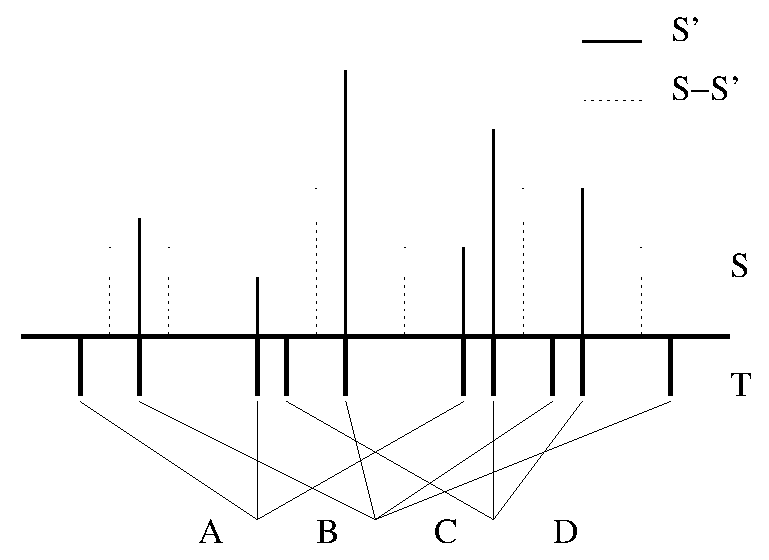
\includegraphics[width=0.6\textwidth]{./img/spectrum_sigma_theta.eps}
\caption{\label{fig:spec-ex}
Representation of a hypothetical target spectrum $\Sigma$ of experimental peaks
$x_i=(\rho_i,I_i)$, matched by the theoretical peaks of $\Theta$,
produced by the amino acid sequence $P=ABCD$.
In the figure the subset $\Sigma'$ represent the experimental peaks matched by
at least one theoretical peak.}
\end{center}
\end{figure}

We have seen in table \ref{tab:list} in section \ref{sec:shannon} of chapter
\ref{chap:db}, that CID fragmentation yields several different ion types:
$a,b,c,x,y,z$, with different charges and possible neutral losses. 
However, it 
is not expected, a priori,  that the full list of ions is produced at every fragmentation 
site, since the number and intensities of the
produced peaks greatly depend on different factors, including the three dimensional structure of
the peptide during fragmentation, or the instrument type.
For this reason, let's define  $\Theta_\nu$, a subset of $\mathcal T_\nu$,  as
the ions that have actually been generated from fragmentation at $\nu$, during
the experiment.
The corresponding collection of ions generated at any position will be
$\Theta=\{\Theta_{\nu_k}, k=1,\dots,L-1\}$. 
Any ion in $\Theta$ is characterized by a  mass-over-charge ratio $\rho$,
representing a theoretical peak position; to test the correspondence between
experimental  ($\Sigma$) and theoretical ($\Theta$)
spectra, we define the \emph{image} of a peak $s_i(\nu_k)$ in the spectrum $\Sigma$ as:
\begin{equation}
\mathcal I(s_i(\nu_k)):
\left\{
\pi\in\Sigma |
d\big(\rho(\pi),\rho(s_i(\nu_k))\big)<d_0
\right\}
\label{eq:map}
\end{equation}
where $d$ is the distance between the positions ot the experimental and
theoretical peaks (we will simply choose  $d(\rho_1,\rho_2)=\vert \rho_1-\rho_2\
vert $),  and $d_0$ is a cutoff distance, that we will take to depend linearly
on the position  of the product ion $\rho$, since it is  a reasonable hypothesis
that the errors on a spectral measure
are also proportional to the mass. %.value of the product ion $\rho$.
With this assumption we take %introduce a distance cutoff dependant on the peak's mass-to-charge value: 
$d_0= min(\gamma_1,\rho(s_i(\nu_k)) \gamma_2)$,
where the parameters $\gamma_1$ and $\gamma_2$ are empirically chosen with the
values $\gamma_1=2.0$ and $\gamma_2=0.0006$.

 Notice that in Eq.~\ref{eq:map} the image of a fragment could be represented by
several peaks, or also be the null set $\emptyset$. We then define
% The previous assumptions, and the definition of matching peaks defined on
% \ref{eq:map}, lead to the definition of a subset of $\Sigma$ and $\Theta$ with
% matched and matching peaks. 
%We define then
the subset $\Theta'_\nu$ of $\Theta_\nu$,  composed of  the
theoretical ions  produced in the fragmentation at $\nu$, that effectively match
at least one peak from the real
spectrum $\Sigma$:
\begin{equation}
\Theta'_\nu=%\Theta'_\nu(\Sigma,\Theta_\nu)=
\left\{
s_i(\nu)\in\Theta_\nu \vert
\mathcal I(s_i (\nu)) \neq \emptyset
\right\}
\end{equation}
Analogously,  the subset of the experimental spectrum $\Sigma$ of peaks that are the image of 
%matched by 
the theoretical peaks of $\Theta'_\nu$ can be defined as:
\begin{equation}
\Sigma'_\nu=%\Sigma'_\nu(\Sigma,\Theta'_\nu)=
\left\{
\mathcal I(s_i(\nu)) \vert s_i(\nu)\in\Theta'_\nu \right\}
\end{equation}
The corresponding global sets: $\Theta'=\{\Theta'_{\nu_k}, k=1,\dots,L-1\}$ and
$\Sigma'=\{\Sigma'_{\nu_k}, k=1,\dots,L-1\}$ are defined as before.

We observe that  the experimental peaks in  $\Sigma'$ need not necessarily be
the real image of the corresponding theoretical fragment:
% Theoretical peaks expected from the fragmentation at the peptide bond in $\nu$
% and that effectively match a experimental peak (those that compose
% $\Theta'_\nu$) can be interpreted in two different ways: the experimental peak
% is indeed the expression of the fragmentation event and in particular of the ion
% species $s_\nu$; on the other hand, 
indeed, if several experimental peaks can match the same fragment ion at $\nu$,
at most one of them will be  the real image of the fragment, the rest being a
product of noise. However,
there is also  the possibility that the ion $s_i$ was not recorded for some
reason, and all the experimental
matching  peaks  are a product of noise. Finally,   both $P$ and the noise could
contribute to the observed intensity of the same peak.
To deal with this possibilities, we introduce the concept of \emph{expressed peak}, referring to 
%We call \emph{expressed peaks} 
those ions of $\Theta'_\nu$ that effectively
produced a peak in $\Sigma'_\nu$:
\begin{equation}
\mathcal E(s_i(\nu))=
\left\{
\begin{aligned}
&1&&\textrm{if}\ \exists\ \pi\in\Sigma'_\nu|s_i(\nu)\to\pi\\
&0&&\textrm{otherwise}
\end{aligned}
\right.
\end{equation}
%With this interpretation in mind one can then 
and we define last two subsets of
$\Sigma$ and $\Theta$ with the expressed ions and the corresponding experimental
peaks:  (even if we might not be able to identify them among the others):
\begin{align}
\Theta''_\nu %=\Theta''_\nu(\Sigma,\Theta'_\nu)
&=
\left\{
s_i(\nu) \in \Theta'_\nu | \mathcal E(s_i(\nu))=1\right\}\\
\Sigma''_\nu&=
\left\{
\mathcal I(s_i(\nu)) | s_i(\nu)\in\Theta''_\nu
\right\}
\end{align}


% Can occur that a theoretical ion matches two or more real peaks, in this case it is more likely
% that only one represents the ion expression while the others are just noise.
% We can not distinguish \emph{a priori} which of them represents a fragment and
% which represents instrument noise (we will later introduce a \emph{a posteriori}
% selection rule).

%\begin{figure}
%\centering
%\begin{pspicture}(0,0)(8,-6)
%%\psgrid(0,0)(0,0)(8,-10)
%\rput(4,-1){\rnode{T}{\psframebox{$\Theta\equiv P$}}}
%\rput(4,-2.5){\rnode{T1}{\psframebox{$\Theta'$}}}
%\rput(3,-2.5){\rnode{T11}{\psframebox{$\Theta'$}}}
%\rput(2,-2.5){\rnode{T12}{\psframebox{$\Theta'$}}}
%\rput(1,-2.5){\rnode{T13}{\psframebox{\dots}}}
%\rput(4,-5.5){\rnode{T2}{\psframebox{$\Theta''$}}}
%\rput(6,-1){\ovalnode{S}{$\Sigma$}}
%\rput(6,-4){\ovalnode{S1}{$\Sigma'$}}
%\rput(6,-5.5){\ovalnode{S2}{$\Sigma''$}}
%\ncline[nodesepB=1pt]{->}{T}{T1}
%\ncline[linestyle=dashed,nodesepB=1pt]{->}{T}{T11}
%\ncline[linestyle=dashed,nodesepB=1pt]{->}{T}{T12}
%\ncline[linestyle=dashed,nodesepB=1pt]{->}{T}{T13}
%\ncline[nodesepB=1pt]{->}{T1}{S1}
%\ncline[nodesepB=1pt]{->}{S}{S1}
%\ncline[nodesepB=1pt]{->}{S1}{S2}
%\ncline[nodesepB=1pt]{->}{S1}{T2}
%\ncline[nodesepB=1pt]{->}{T1}{T2}
%\end{pspicture}
%\caption{\label{fig:sets}caption}
%\end{figure}

To avoid to deal with mixed situations as those described above, we can assume that:
\begin{hypothesis}
If $\pi$ is a experimental peak of $\Sigma''$, we assume that it is entirely due
to the corresponding species $s_i\in\Theta''$
\end{hypothesis}
Also, we assume that:
\begin{hypothesis}
The chances of multiple matches to the same experimental peak $\pi$ by different
fragment ions are negligible.
\end{hypothesis}
The above defined sets imply that all the peaks in $\Sigma \setminus \Sigma''$
are a product of noise, and that all the fragment ions in 
$\Theta'\setminus \Theta''$ have not produced any peak in the spectrum.
% 
% Some further remarks on those sets. The set of
% matched peaks $\Sigma'_\nu$ is completely defined from the definition of the
% spectrum $\Sigma$ and the matchable peaks $\Theta'\nu$. 
% This does not represent a
% one-to-one correspondence between $\Theta'_\nu$ and $\Sigma'_\nu$ as there can be some
% matchable peaks that actually do not match any experimental peak
% $\Theta'_\nu\setminus\Theta''\nu$; moreover some matchable fragments can actually match
% more than only one real peak if they fall \emph{near} the theoretical expected
% $\rho$.
% 
% We face also to some rare event like a peak from the spectrum is mathched by
% more then one expected ion from the peptide.
% We consider as negligeble this event:

%As reported previously, from the latter we will select one and only one
%experimental peak that will be the product of matchable theoretical ion.

\section{Protein sequencing as a an inference problem}

%\section{An Insight into the Probability}

 Let us consider the problem of spectra interpretation as a Bayesian inference
problem. We have seen that three different elements are involved in the MS/MS
experiment, 
$P$, $\Sigma$ and $R^\Sigma$, that can be considered as random variables,
extracted from different distributions.
Their joint probability  $p(P,R^\Sigma, \Sigma)$ can be
written as: %ans hypothesis \ref{hyp:p-r} as:
\begin{align}
p(P,R^\Sigma,\Sigma)&=p(\Sigma \vert P,R^\Sigma)p(P, R^\Sigma)\\
&= p(P \vert \Sigma, R^\Sigma)p(\Sigma, R^\Sigma)
\label{eq:p1}
\end{align}
introducing the conditional probabilities $p(\Sigma \vert P,R^\Sigma)$ of
observing the spectrum $\Sigma$ given the parent sequence $P$ and the source
$R^\Sigma$, and $p(P \vert \Sigma,R^\Sigma)$ of the parent sequence $P$ given
the observed spectrum $\Sigma$  and the noise  $R^\Sigma$.

We assume that the events generating spectrum noise are completely independent from
the precursor ion  and the fragmentation process that produce the true peaks:
\begin{hypothesis}
$R^\Sigma$ is uncorrelated from the peptide sequence $P$:
$p(P,R^\Sigma)=p(P)p(R^\Sigma)$.
\label{hyp:p-r}
\end{hypothesis}
% We consider then the join probability $p(P,R^\Sigma, \Sigma)$ which can be
% written using Bayesian rules ans hypothesis \ref{hyp:p-r} as:
% \begin{equation}
% p(P,R^\Sigma,\Sigma)=p(\Sigma|P,R^\Sigma)p(P)p(R^\Sigma)
% \label{eq:p1}
% \end{equation}

We also consider the noise distribution to be the same for every spectra, and to
be independent from the \emph{a-priori} distribution of the spectra:
\begin{hypothesis}
$R^\Sigma$ is independent from the target spectrum
$\Sigma$: $R^\Sigma\approx R\quad \forall \Sigma$, and
$p(R^\Sigma,\Sigma)\approx p(R)p(\Sigma)$.
\label{hyp:r-s}
\end{hypothesis}

Our goal is to estimate the posterior probability $p(P\vert R,\Sigma)$ that the
peptide $P$ is the precursor ion, given the experimental spectrum $\Sigma$ and
noise distribution $R$. However, we observe that in any \emph{de-novo} framework
the actual sequence $P$ cannot be resolved by the experiment, because of the
possible  mass degeneracies as between Isoleucine and Leucine: for instance, in
our modelling scheme, peptides differing by these residues at the same position
would correspond to the same configuration of our one-dimensional system,
characterized by the same set of fragmentation sites $\mathcal F(P)$ and
corresponding theoretical ions
we are interested in determining $\mathcal T(P)$ from the MS/MS data, since
$\mathcal T(P)$.
% 
% Moreover, we note that the correspondence between $P$ and the set of corresponding theoretical ions $\mathcal T(P)$
% is not one-to-one, at difference from the relation between the theoretical ions  $\mathcal
% T(P)$ and the fragmentation sites %peptide bond sites 
% $\mathcal F(P)$.
% Indeed,  the same set $\mathcal T(P)$ can correspond to several precursor sequences $P$, due to the degeneracy between 
% % the case, for example, of sequences containing 
% Leucine and Isoleucine. 
On the other hand, once given $P$,  the sets $\mathcal F(P)$ and $\mathcal T(P)$
are completely determined.
Therefore we can write, for any random variable $Y$:
\begin{equation}
p(P \vert Y)\equiv p(P,\mathcal T(P)\vert Y)=p(P|\mathcal T(P), Y)p(\mathcal T(P)\vert Y)
\label{eq:p-t}
\end{equation} 

This is true in particular for 
\begin{equation}
 p(P \vert R,\Sigma)=p(P \vert \mathcal T(P)) p(\mathcal T(P)\vert R,\Sigma)\,.
\label{eq:goal}
\end{equation}
where we have used the fact that  $ p(P \vert \mathcal T(P), \Sigma, R)=p(P
\vert \mathcal T(P))$, since no extra information about $P$, with respect to the
one contained in $\mathcal T(P)$, is carried by $\Sigma$ or $R$.
So, Equation \ref{eq:p1}, using Equations \ref{eq:p-t}, \ref{eq:goal} and hypothesis
\ref{hyp:r-s} can be rewritten in the following way:

\begin{align}
p(P,R,\Sigma)&=p(\Sigma \vert P,R) p(P|\mathcal T(P)) p(\mathcal T(P)) p( R)\\
&= p(P \vert \mathcal T(P)) p( \mathcal T(P) \vert \Sigma, R)  p(\Sigma) p(R)
\label{eq:p2}
\end{align}
% 
% \begin{equation}
% p(P,R,\Sigma)=p(P|\mathcal T(P),R,\Sigma)p(\mathcal T(P)|R,\Sigma)p(R)p(\Sigma)
% \label{eq:p2}
% \end{equation}
% that
% in the sequence $P$ itself because degeneracies as Leu-Ile cannot be resolved in
% the mass spectrometry framework.

Thus, %using equations \ref{eq:p1} and 
from Eq. \ref{eq:p2} one can finally write:
\begin{equation}
p(\mathcal T(P)\vert R ,\Sigma)=
p(\Sigma\vert P,R)
\frac{p(\mathcal T(P))}{p(\Sigma)}
\label{eq:start}
\end{equation}
which expresses Bayes theorem, and will be our starting point in the following. 
%of our implementation, searching 
Interpreting the spectrum will be equivalent to finding the peptide
sequence $P'$ that maximize probability \ref{eq:start}:
\begin{equation}
P'=\underset{P}{\text{argmax}}[p(\mathcal T(P)\vert R,\Sigma)]=
\underset{P}{\text{argmax}}[p(\Sigma|P,R)p(\mathcal T(P))]\,\,,
\label{eq:bestP}
\end{equation}
where we neglect the denominator, which is the same in all the maximization
process. Such $P'$ is the best prediction we can give of the true precursor ion
$P^*$.

In the above expression, $p(\mathcal T(P))$ is unknown, but some reasonable
assumptions can be made on it, basing, for instance, on the amino acid
frequencies, or on some other \emph{a-priori} information on the system under study.
The key point is, however, how to estimate the probability $p(\Sigma \vert P,
R)$ that, given a sequence $P$, (represented by its set of theoretical fragments
$\mathcal T(P)$ encoded in the state variables of our model) and a source of
statistical noise $R$, we will observe the experimental spectrum $\Sigma$.

If the physics of the fragmentation process in CID was well understood, along
with the distribution of contaminants and other factors responsible for the
noise peaks of a spectrum, we could calculate,  for any individual parent
peptide molecule, the probability of fragmentation $p^{\texttt{true}}(s_i|P)$
at any site , involving the generation of any ion species $s_i$. Such
probability, together with the corresponding one, $p(\rho|R)$, that the noise
$R$ is contributing at position $\rho$,  would allow to calculate the true
$p(\Sigma \vert P, R)$ for any $P$
%Such probability would be directly proportional to the corresponding peak intensities, so that,
% given a parent peptide and a model for the contaminants intervening in its
% measure, a theoretical spectrum could be associated to any experimental setup
% and precursor peptide.
Identification would then proceed by comparing the experimental spectrum with
the theoretical ones associated to all the possible parent peptides, and
choosing the peptide whose theoretical spectrum is most similar to the
experimental one (using some suitable measure of similarity, as for instance
Kullback-Leibler distance). In this approach, the theoretical spectra would be
calculated from first principle, with a ``true'' Hamiltonian function, and the
information from the experimental spectrum would be used a posteriori, in the
comparison of the average intensities.

The lack of a suitable \emph{ab-initio} Hamiltonian to describe the
fragmentation process prompts for a different approach, where information
proceeding from the experimental spectrum itself, or by the typical peak
distributions in a database of spectra, is used to derive an ad-hoc energy
function, so that the experimental spectrum acts as an ``external field''
biasing the system towards the most-likely parent peptide sequence.

We will use the latter approach here, which is common to all \emph{de-novo}
methods. We will also adopt a different view on the MS/MS spectra generation:
instead of considering a spectra  as the outcome  from an ensemble of molecules,
and of describing the fundamental process as the fragmentation of one single
molecule into two pieces during CID,  we will consider the whole spectrum as the
overlap between the signal from a noise source and from the fragmentation in
multiple sites of a unique parent sequence, both of them generating peaks ``as a
whole'', with a characteristic position and intensity $(\rho,I)$.
In other words, due to our ignorance of the true energy function underlying the
spectra generation, we move away from the (physically correct) view of a MS
spectrum as the overlap between the weak signals of an ensemble of individual
products ions, and adopt a more bioinformatics-oriented view of a spectrum
generated by a unique entity, yielding several ion products at each
fragmentation site $\nu$, that are rewarded or penalized according to an
external empirical potential, based on our results of the previous chapter, on
the distribution of probability of the peaks in the $(\rho,I)$ plane. This
approach allows us to reward the presence in the spectrum of several ion species
representing fragmentations at the same position along the sequence (e.g,
detection of $y$ $b$, etc. ions originating from fragmentations at the same
position $\nu$).

To define the energy function, we need to develop Eq.~\ref{eq:start} in finer detail.



Let us call $\mathcal A^\Sigma(P)$ an assignment of the sequence $P$ on the
spectrum $\Sigma$, specifying which theoretical ions $\Theta$ were actually
produced, which of them $\Theta''$  were  detected, and which were the
corresponding peaks $\Sigma''$ in the spectrum:
\begin{align}
\mathcal A^\Sigma(P)=\{\Theta,\Theta'',\Sigma''\}&\equiv
\{\Theta,\Theta'',\Sigma'';\Theta\setminus\Theta''\}
\label{eq:assignment}
% \\
% \intertext{where}
% \Theta''&=\bigcup_{\nu\in\mathcal F(P)} \Theta''_\nu\\
% \Sigma''&=\bigcup_{\nu\in\mathcal F(P)} \Sigma''_\nu
\end{align}
The last expression underlines that, given $\Theta$  and $\Theta''$, the set of
fragmentations that have not produced a peak in the spectrum is also completely
determined as $\Theta\setminus\Theta''$.



The probability $p(\Sigma|P,R)$ can be written as the sum over the different
ways that spectrum peaks can be assigned to the sequence $P$:
%is this case calculated in term of assignment
% as in \ref{eq:assignment} that interprets in different ways the association of
% theoretical peaks calculated from the proposed sequence $P$ and the spectrum
% peaks.
% The equation \ref{eq:start} takes the form:
\begin{align}
p(\Sigma|P,R)&=
\sum_{\mathcal A^\Sigma(P)}
p(\Sigma,\mathcal A^\Sigma(P)|P,R)=\\
&=
\sum_{\mathcal A^\Sigma(P)}
p(\Sigma|\mathcal A^\Sigma(P),P,R)
p(\mathcal A^\Sigma(P)|P,R)
\label{eq:assign_sum}
\end{align}
where the sum over $\mathcal A^\Sigma(P)$ involves all possible choices of  $\Theta \subset \mathcal
T$, $\Theta''\subset \Theta'$ and $\Sigma''\subset \Sigma'$.
As we mentioned, 
this implies that there may be some theoretical ions $s\in\Theta'\setminus\Theta''$
that are considered to have escaped detection, and %, even if they could be matching %, while they are matching 
if any peaks  of the spectrum could match them, the latter are considered as noise.
Moreover, this also implies that when  a single theoretical ion $s$ can match more
than  one spectrum peak, the sum also involves all the way the ``true'' image of $s$ can be chosen in $\Sigma'$.
To simplify the approach we introduce two hypotheses:
\begin{hypothesis}
If an ion species $s\in\Theta'$ can match an experimental peak $\pi\in\Sigma$,
then the peak should be interpreted as the image of $s$.
\label{hyp:theta2}
\end{hypothesis}
\begin{hypothesis}
If an ion species $s\in\Theta'$ matches more than one experimental peak in $\Sigma$,
then the true image of $s$ will be the peak $\pi$ that maximize the probability
(at fixed $\Theta$ and $\Theta''$).
\label{hyp:sigma2}
\end{hypothesis}
On the basis of the hypothesis \ref{hyp:theta2}, we can say that
$\Theta''\equiv\Theta'\subseteq\Theta$. From the hypothesis \ref{hyp:sigma2} it
follows that the peak set $\Sigma''$ is completely determined by the definition
of $\Sigma,\Theta$ and $\Theta''$.
Following previous hypothesis (\ref{hyp:theta2} and \ref{hyp:sigma2}), 
the sets $\Theta''$ and $\Sigma''$ in the assignment $\mathcal A^\Sigma(P)$
remains completely determined  once defined the set  $\Theta$, so that the sum
in Eq.~\ref{eq:assign_sum} is simplified:
\ref{eq:assign_sum} change to:
\begin{equation}
p(\Sigma|P,R)=
\sum_{\Theta\in\mathcal T(P)}
p(\Sigma|\mathcal A^\Sigma(P),P,R)p(\mathcal A^\Sigma(P)|P,R)
\label{eq:sigma_sum}
\end{equation}
The probability $p(\Sigma|\mathcal A^\Sigma(P),P,R)$, given the assignment
$\Theta,\Theta''$ and $\Sigma''$, corresponds to the probability that
the remaining unassigned peaks in $\Sigma\setminus\Sigma''$ are due
to noise. Under the hypothesis:
\begin{hypothesis}
Peaks due to noise are independent random events;
\label{hyp:indipR}
\end{hypothesis}
such probability can be factorized as:
\begin{equation}
p(\Sigma|\mathcal A^\Sigma(P),P,R)=
p(R\to\Sigma\setminus\Sigma''|R)=
\prod_{\pi\in\Sigma\setminus\Sigma''}
p(R\to\pi|R)
\end{equation}
The probability of the assignment
$\mathcal A^\Sigma(P)$ is independent from the noise events and thus $p(\mathcal
A^\Sigma (P)|P,R)\equiv p(\mathcal A^\Sigma(P)|P)$.

It would be desirable to propose a factorized form also for the latter probability. 
However, the events that underlie the assignment of the theoretical peaks in
$\Theta''$ to the experimental peaks of $\Sigma''$ are correlated and cannot be
factorized on each $\nu$: for instance the probability of having a peak
corresponding to the ion $s_i(\nu_1)$ and that of a peak from ion $s'_i(\nu_2)$
are not independent. However, we can restrict our attention only to the
fragmentation sites of $P$, and not to all $\nu$, and assume that in this case:
\begin{hypothesis}
Probabilities of different fragmentation sites are independent and can be
factorized on $\nu\in\mathcal F(P)$.
\end{hypothesis}
\begin{hypothesis}
Within a given choice of ion species $\Theta_\nu\subseteq\mathcal T_\nu(P)$
produced in $\nu$, the probabilities are independents and can be factorized on
$s_i(\nu)$.
\end{hypothesis}

With this hypotheses we can rewrite Equation \ref{eq:sigma_sum} as:
\begin{multline}
p(\Sigma|P,R)=
\sum_{\Theta\subseteq\mathcal T(P)}
\left[
\prod_{\pi\in\Sigma\setminus\Sigma''}
p(R\to\pi|R)
\right]\times\\
\times\prod_{\nu\in\mathcal F(P)}
\left\{
\left[
\prod_{s_i(\nu)\in\Theta'_\nu}
p^\text{loc}(s_i\to\Sigma''(s_i),s_i\in\Theta_\nu,s_i\in\Theta'_\nu|P)
\right]
\right.\\
\left.
\left[
\prod_{t_\nu\in\Theta\setminus\Theta'_\nu}
p^\text{loc}(t_\nu\to\emptyset,t_\nu\in\Theta_\nu,t_\nu\in\Theta\setminus\Theta'_\nu|P)
\right]
\right\}
\end{multline}
where $p^\text{loc}(*)$ indicates that the probability is normalized in a small
neighborhood of the theoretical position $\rho(s_i(\nu))$, according
to the fact that, once determined the precursor peptide $P$, the fragmentation
sites $\nu\in\mathcal F(P)$ and then the expected ions $s_i$ are completely
fixed. 

We can then write:
\begin{multline}
p(\Sigma|P,R)=
\Bigg\{\prod_{\nu\in\mathcal F(P)}
\Bigg[\sum_{\Theta_\nu\in\mathcal T_\nu(P)}
\prod_{s_i(\nu)\in\Theta_\nu}\Big(
(1-\delta_{\mathcal I(s_i),\emptyset})w^M(s_i,\mathcal I(s_i))+\\
+\delta_{\mathcal I(s_i),\emptyset}w^{\bar M}(s_i)
\Big)\Bigg]\Bigg\}\times
p(R\to\Sigma)
\label{eq:psigma}
\end{multline}
where
\begin{align}
w^M(s_i,\mathcal I(s_i))&=
\frac{p^\text{loc}(s_i\to\Sigma''(s_i),s_i\in\Theta_\nu,s_i\in\Theta'_\nu|P)}
{p(R\to\Sigma''(s_i)|R)}\\
w^{\overline M}(s_i)&=
p^\text{loc}(s_i\to\emptyset,s_i\in\Theta_\nu,s_i\in\Theta_\nu\setminus\Theta'_\nu|P)\\
p(R\to\Sigma)&=
\prod_{\pi\in\Sigma} p(R\to\pi|R)
\label{eq:wM}
\end{align}
we introduce the dynamical variable $\xi_\nu^{s_i}$ that indicate if there
fragmentation of the peptide in $\nu$ produced the ion $s_i$ or not:
\begin{equation}
\xi_\nu^{s_i}=\left\{
\begin{aligned}
&1 && \text{if\ } s_i\in\Theta_\nu\\
&0 && \text{if\ } s_i\in\mathcal T_\nu\setminus\Theta_\nu
\end{aligned}
\right.
\end{equation}
that let us write equation \ref{eq:psigma} as:
\begin{multline}
p(\Sigma|P,R)=
p(R\to\Sigma)\times
\Bigg\{\prod_{\nu\in\mathcal F(P)}
\prod_{s_i\in\mathcal T_\nu(P)}\Bigg[
\sum_{\xi_\nu^{s_i}=0,1} \Bigg( 
\delta_{\xi_\nu^{s_i},0}+ \\
+\delta_{\xi_\nu{s_i},1}\Big(
(1-\delta_{\mathcal I(s_i),\emptyset})w^M(s_i,\mathcal I(s_i))
+\delta_{\mathcal I(s_i),\emptyset}w^{\bar M}(s_i)
\Big)
\Bigg)
\Bigg]\Bigg\}
\end{multline}

Finally, we go back to Eq.~\ref{eq:start} and we make another assumption on the
\emph{a-priori} probability of the theoretical fragments:
\begin{hypothesis}
The probability $p(\mathcal T(P))$ of the set of theoretical ions from peptide
$P$ can be factorized on individual ions, as independent statistical events; the
\emph{a-priori} probability of any fragment $s_i$  is independent from its type:
\end{hypothesis}
Hence,
\begin{equation}
p(\mathcal T(P))=\prod_{\nu\in\mathcal F(P)}
\prod_{s_i\in\mathcal T_\nu(P)} p_\text{ion}
\end{equation}
where $p_\text{ion}$ is a constant for all fragmentation sites $\nu$ and species
$s_i$.

In the end, our proposal for the posteriori probability  of observing $P$ as the
parent peptide, given the experimental spectrum $\Sigma$ and a model $R$ for the
noise, is given by Eq.~\ref{eq:goal} together  with
Eq.~\ref{eq:bestP} and:
\begin{multline}
p(\mathcal T(P)\vert \Sigma, R) \propto
p(R\to\Sigma)\times
\Bigg\{\prod_{\nu\in\mathcal F(P)}
\prod_{s_i\in\mathcal T_\nu(P)}
p_{\text{ion}}
\Bigg[
\sum_{\xi_\nu^{s_i}=0,1} \Bigg( 
\delta_{\xi_\nu^{s_i},0} +\\
+\delta_{\xi_\nu^{s_i},1}\Big(
(1-\delta_{\mathcal I(s_i),\emptyset})w^M(s_i,\mathcal I(s_i))
+\delta_{\mathcal I(s_i),\emptyset}w^{\bar M}(s_i)
\Big)\Bigg)
\Bigg]\Bigg\}
\label{eq:finalp}
\end{multline}


%------------------------------------------------------------------

\section{An empirical Energy Function}
\label{potential}
Equation \ref{eq:finalp} provides us with a recipe to evaluate the fitness of
any sequence $P$ to match the spectrum $\Sigma$, as a product over all the
fragmentation sites $\nu \in \mathcal F(P)$ of $P$, and over all the possible
theoretical fragment ions that could in principle be generated by sequence $P$,
of the probability to generate any fragment, times a term accounting for all the
possible patterns in which the ions  $s_i$ can be  actually generated, and, if
they are, weighting the probability to have generated a peak in the spectrum
($w^M$), or to have produced no peak ($w^{\bar M}$).
The above expression is further multiplied by the probability $p(R\to\Sigma)$
that the whole spectrum is generated by the noise. The latter term is
independent from the parent sequence, so that we can ignore it in the following,
and keep the rest of the expression as a guide to introduce an ad-hoc
Hamiltonian for our model, by writing:
\begin{equation}
p(\mathcal T(P)\vert \Sigma, R) \propto
\Bigg\{\prod_{\nu\in\mathcal F(P)}
\Bigg[
\prod_{s_i\in\mathcal T_\nu(P)}
\left(
\sum_{\xi_\nu^{s_i}=0,1} e^{-\beta H(\nu,s_i,\xi_\nu^{s_i})}
\right)
\Bigg]\Bigg\} \,\,,
\end{equation}
where $\beta$ is a fictitious inverse temperature, and  we have introduced:

\begin{multline}
H(\nu,s_i,\xi_\nu^{s_i})=\mu-\delta_{\xi_\nu^{s_i},1} 
\Big(
(1-\delta_{\mathcal I(s_i),\emptyset}) \log (w^M(s_i,\mathcal I(s_i))+\\
+\delta_{\mathcal I(s_i),\emptyset} \log (w^{\bar M}(s_i))
\Big)\,,
\label{eq:Ham}
\end{multline}
defining the chemical potential as $\mu=-\log p_{\text{ion}}$.

This corresponds to defining the energy function in terms of the probabilities
contained in the expressions of $w^M$ and $w^{\bar M}$ in Eq.~\ref{eq:wM}, that
are, however, unknown. We propose an empirical estimate for such quantities
resorting to the results of chapter \ref{chap:db}, on the
phenomenological distributions obtained by the analysis of a large  database of
spectra with the associated predicted precursor ion.

Namely, in order to define the probability of matching a real peak
$p^\text{loc}(s_i\to\Sigma''(s_i),s_i\in\Theta_\nu,s_i\in\Theta'_\nu|P)$
and the probability of a theoretical ion to not match any experimental peak
$p^\text{loc}(s_i\to\emptyset,s_i\in\Theta_\nu,s_i\in\Theta\setminus\Theta'_\nu|P)$,
we express them in term of database frequencies.
The former represents the probability that, given the fragmentation site 
$\nu\in\mathcal F(P)$, the dissociation event produced the species $s_i$ and
this was detected as a peak in the final spectrum.
In a similar way, the latter represents the probability that, given
$\nu\in\mathcal F(P)$, the species $s_i$ was produced, but for some reason it
did not yield any peak in the experimental spectrum.
We express these probabilities as:

\begin{align}
p^\text{loc}(s_i\to\Sigma''(s_i),s_i\in\Theta_\nu,s_i\in\Theta'_\nu|P)
&=
\frac{N(s_i,x(\Sigma''(s_i)))}
{\displaystyle
\sum_{t\in\mathcal T_\nu(P)}N^T(t,\mathcal J_\delta(\rho(t)))}
\\
p^\text{loc}(s_i\to\emptyset,s_i\in\Theta_\nu,s_i\in\Theta\setminus\Theta'_\nu|P)
&=
\frac{N(\bar s_i,\mathcal J_\delta(\rho(s_i)))}
{\displaystyle
\sum_{t\in\mathcal T_\nu(P)}N^T(t,\mathcal J_\delta(\rho(t)))}\\
p(R\to\pi|R)
&=
\frac{N(R,x(\pi))}{N(R)}
\end{align}
where $x(\pi)$ represents the cell in which the peak $\pi$ fall, in the cell the
distribution of peaks is taken as constant; $\mathcal J_\delta(\rho)$ represents
the interval $[\rho-\delta,\rho+\delta]$ and considers all peak intensity
values.
$N(x,y)$ represents the frequency of peaks matched as $x$ inside the interval
$y\equiv y_\rho\times y_I$ and $N(\bar x,y_\rho)$ the number of absent $x$ type
ions in the interval $y_\rho$, while $N^T(x,y_\rho)$ represent the expected number of peaks $x$ in the
$y_\rho$ interval of the $\rho$ axis accounting for both matched and absent peaks:
$N^T(x,y_\rho)= N(\bar x,y_\rho)+\sum_I N(x,y_\rho\times y_I)$.

 Finally, we note that also the value of the
\emph{chemical potential} $\mu$ defined above is unknown. 
We observe that its practical role is to penalize the system against matching
the experimental spectrum with too many fragment ions, i.e., using sequences
with the highest allowed  number of residues (and fragmentation sites),
polarizing the result towards the lightest residues, ending up in an excess
of Glycines.
For this reason, we fix it 
\emph{a posteriori}, optimizing the agreement between the predicted peptide and
the ``true'' parent, as predicted  by SEQUEST, for the spectra in the learning
database.

